\section{Background}
\justify
This chapter describes the main concepts related to the project work. Firstly,
the chapter provides the definition and example of embedded systems. Then, it
introduces the Bluetooth Low Energy along with some common concepts. Finally,
the last two sections provide an overview of the project and the chosen hardware.

\subsection{Embedded systems}
\justify
The definition of embedded systems varies among people. Some people, who 
work with desktop application or web application, may refer mobile devices 
as an embedded system. Some, however, who has developed application for 
8-bit microcontroller system seem not to agree. Though it is hard to define, 
embedded systems share some common characteristics:
\begin{itemize}
    \item Application-specific: 
        As opposed to general purpose computing device such as personal 
        computer, embedded devices are developed with pre-defined use cases 
        in mind and only offer a limited set of functions.
    \item Real world interaction:
        Embedded systems are developed to solve real world problem. They can
        be used to control some hardware, sense the environment with sensors, 
        or manipulate the physical world with actuators.  
    \item Constraints of hardware: 
        The resources, such as energy, CPU, memory, are limited. There are
        several ways to classify hardware used in embedded systems in terms 
        of resources. For instance, the Internet Engineering Task Force has 
        its own taxonomy of constrained-node networks \cite{BEK14}: 
        \begin{itemize}
            \item Class 0 devices have smallest resources, typically 
                $\ll$ 10 KiB of RAM and $\ll$ 100 KiB of Flash size.
            \item Class 1 devices have medium-level resources, typically 
                $\sim$ 10 KiB of RAM and $\sim$ 100 KiB of Flash size.
            \item Class 2 devices have more resources, typically 
                $\sim$ 50 KiB of RAM and $\sim$ 250 KiB of Flash size. 
        \end{itemize}
    \item Constraints of software: 
        Some systems require the software must act deterministically, soft 
        real-time, or hard real-time. Other systems require that the software
        be fault-tolerant in the face of errors (e.g., flight control systems
        on airplane) or to cease the operation at the first sign of problem (e.g.,
        medical devices). \cite[p.~1]{White11} 
\end{itemize}
An example of an embedded device is shown in figure 1, an IoT sensor kit named
Nordic Thingy:52. This is an easy-to-use prototyping platform helping in rapidly
building prototypes and demos \cite{Thingy19}. 
\begin{figure}[H]
    \centering
    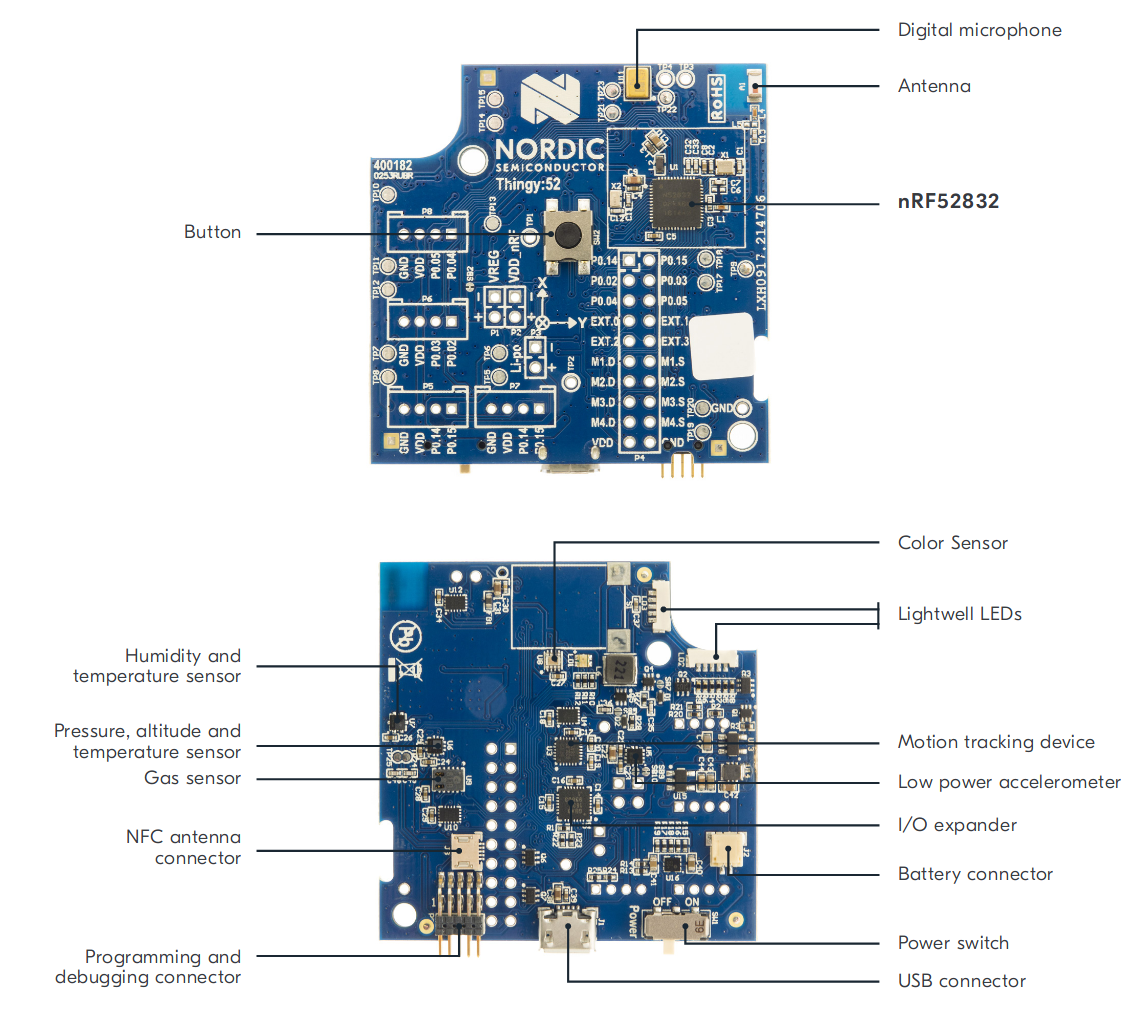
\includegraphics[scale=1.6]{figure/figure01_thingy_52.png}
    \caption{Nordic Thingy:52. Adapted from \cite{Thingy19}.}
\end{figure}
\justify
As illustrated in figure 1, Nordic Thingy:52 consists of several components of an
typical embedded system:
\begin{itemize}
    \item Microcontroller/Microprocessor/System-on-Chip (SoC): 
        This is the heart of the system as it glues all components together.
        Its key job is to communicate with sensors for input variables and 
        actuators for output variables as well as processing the data. Other 
        hardware are built into the chip to assist these communication such as 
        analog-to-digital converter, digital-to-analog converter, and so on.

    \item Sensors:
        Each application interests to different set of data for its purposes. 
        The data collected by these sensors serve as the input to the system.
        The example device includes different types of sensors, such as color
        sensor, humidity and temperature sensor, and others.
    \item Actuators:
        In order to manipulate the environment in which the device operates,
        some actuators has to be built into the system. After processing the 
        input data collected by sensors, the cetral controller outputs signal 
        to control some actuators, for instance, LEDs, screen, to perform 
        the desired actions.    
    \item Power supply:
        This is the essential component of the system. Two primary sources of 
        power supply for an embedded system are wall power and batteries. Hence,
        the system could be powered by any one of these models:
        \begin{itemize}
            \item Wall powered
            \item Wall powered with battery as a backup
            \item Battery powered
        \end{itemize}
    \item Interfaces with other systems:
        An embedded system usually has some interfaces to communicate with other
        systems. They can be, for example, programming and debugging interface, 
        or USB port. They are important part of the system not only to the developer,
        who have to use debugging interface to aid the development process, but also
        the user to extend the existing functionalities by incorporating other devices.  
    \item Other application-specific components:
        Some systems require specific components for their application. For example, 
        the nRF52832 SoC needs an external antenna for wireless communication.
\end{itemize}

\subsection{Bluetooth Low Energy (BLE)}
\justify
Bluetooth Low Energy (BLE), also refers to as Bluetooth Smat, is a subset of Bluetooth
classic and was first introduced as part of the Bluetooth 4.0 core specification. It 
was started as an project originally developed by Nokia named Wibree and later being
adopted by the Bluetooth Special Interest Group (SIG). \cite[p.~1]{TCAD14}

% Design goals and features
\justify
The key desgin goals of BLE are robustness, low power consumption, and low cost. It is
intended to replace cables with short-range wireless communications connecting portable
and fixed electronic devices. In addition, the BLE is also designed for use cases and 
application with low data rates and low duty cycles \cite[p.~180]{Ble19}. 
For example, a wireless sensor node with BLE for data transmission, which only activate 
for a few minutes a day, can last for months with a single coin cell battery. 
The most appealing feature of BLE is that most majors platform, as listed below, support
Bluetooth 4.0 and Bluetooth Low Energy:
\begin{itemize}
    \item iOS 5+
    \item Android 4.3+ 
    \item Apple OS X 10.6+
    \item Windows 8,10 
    \item GNU/Linux Vanilla BlueZ 4.93+
\end{itemize}
Hence engineers and product designers can easily develop new products that being able
to talk to any modern computing platform, especially mobile devices. BLE can also lower
the barrier to adopt new products since users have already accustomed to using 
smartphones or tablets, which means the learning curve of using new external devices 
is more gentle \cite[p.~2]{TCAD14}. As a result, BLE exists on most of smart watches 
nowadays for data exchange with users' mobile phones.  

\subsubsection{Configurations and network topology}
A Bluetooth core system consists of a Host and one or more Controllers. It means that
a BLE system can exist with or without Bluetooth classic. The figure 2 depicted two 
types of BLE system.
\begin{figure}[H]
    \centering
    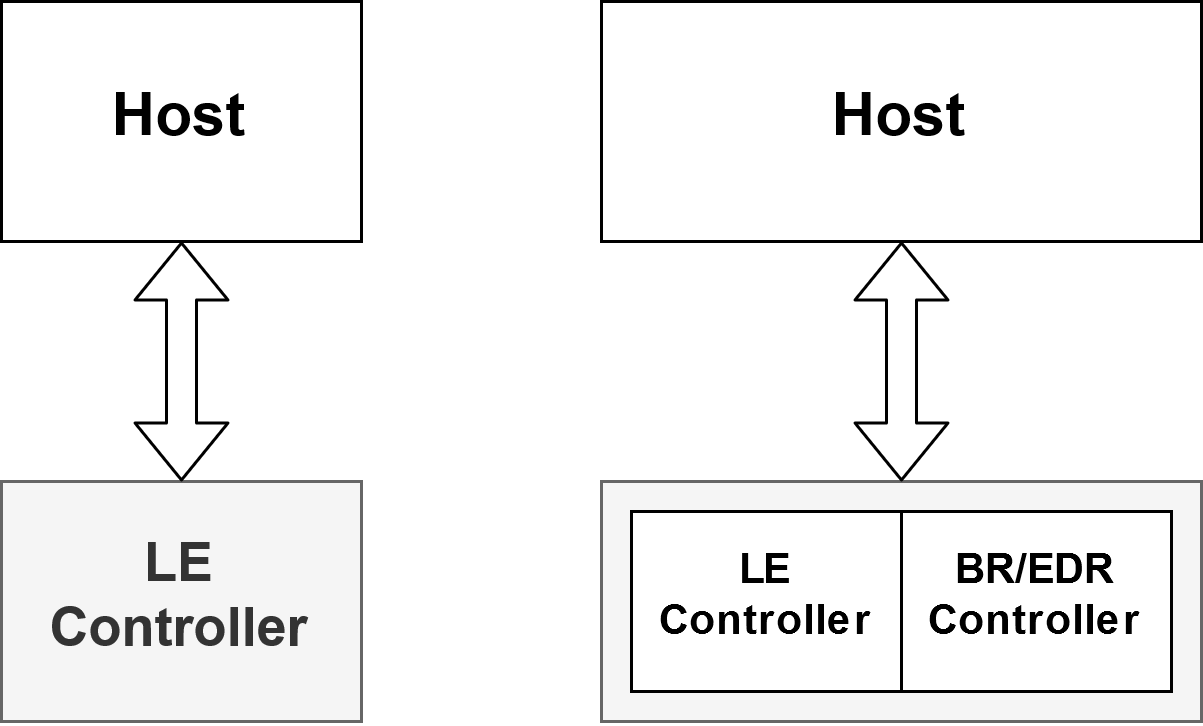
\includegraphics[scale=0.6]{figure/figure02_ble_configurations.png}
    \caption{Configurations for devices with BLE.}
\end{figure}
\justify
A Host is the upper layers in the BLE protocol stack which below the non-core profiles
and above the Host Controller interface (HCI). A Controller is the lower layers in the 
BLE protocol stack including the physical layer (LE PHY), Link Layer and optionally HCI. 
Theses layers can be implemented in a single integrated circuit or they can be split 
and communicate through other protocol (UART, USB, SPI, or other).

\justify
A Bluetooth Low Energy device can communicate with the other peers in two ways: 
broadcasting or connections.
Broadcasting allows the device, which acts as broadcaster, to send one-way data to 
other scanning device or receiver in the listening range, which acts as observer. 
The device broadcasts data by sending advertising packet containing 31-byte payload,
which includes data decribes the device, its capabilities, and other user-defined 
information. BLE also supports a sencondary advertising packet, which is also 31 bytes.
In total, the device can transmit up to 61 bytes to other interested peers without the
need of making connection. However, advertising packets are not encrypted thereforce 
they are not suitable for sensitive data.
In order to transmit data bidirectionally, or a large amount of data, two devices have
to make connection. One device acts as central (master) and initiates the connection
with other device acts as peripheral (slave). Once a connection is established, the
peripheral device stops advertising and both devices can start exchanging data.
The advantages of connections comparing to broadcasting are securities and data 
organisation with services and characteristics.

\subsubsection{The BLE stack}
\justify
The BLE protocol stack is a combination of several layers that provide the 
functionality required to operate. 
\begin{figure}[H]
    \centering
    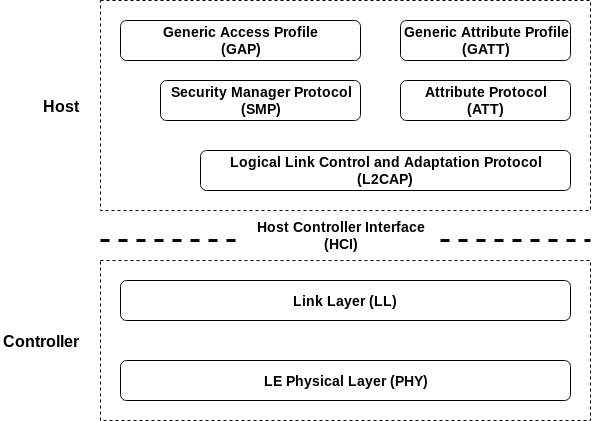
\includegraphics[scale=0.6]{figure/figure03_ble_stack.png}
    \caption{The BLE stack.}
\end{figure}
\justify
As shown in figure 3, each layer belongs to either Host or Controller. 
The HCI is an optional component and appear in both Host and Controller.
\begin{itemize}
    \item Host:
        \begin{itemize}
            \item Generic Access Profile (GAP):
                This layer represents the base functionality common to all 
                BLE devices such as modes and access procedures used by the 
                transports, protocols and application profiles. Its services 
                include device discovery, connection modes, security, 
                authentication, association models and service 
                discovery. \cite[p.~198]{Ble19}
            \item Generic Attribute Profile (GATT):
                This layer represents the functionality of the attribute server 
                and, optionally, the attribute client.
                GATT provide a hierarchy and abtraction model in terms of services,
                characteristics, and attributes for data exchange between devices.
                It provides interfaces for discovering, reading, writing, and 
                indicating of service characteristics and 
                attributes. \cite[p.~198]{Ble19} 
            \item Attribute Protocol (ATT):
                This layer implements the peer-to-peer protocol between an 
                attribute server and an attribute client. To read and write 
                values of attributes on a peer device with an ATT server, the 
                client sends requests to the server and the server sends data 
                to the client. The client can also send commands, and confirmations
                to the server while the server can also send notifications, and 
                indications to the client as well. \cite[p.~198]{Ble19}
            \item Security Manager Protocol (SMP):
                SMP is the peer-to-peer protocol used to generate encryption keys 
                and identity keys. It also manages storage of the encryption keys 
                and identity keys and is responsible for generating random addresses 
                and resolving random addresses to known device identities. 
                During the encryption or pairing procedures, SMP interfaces directly 
                with the Controller to provide stored keys used for encryption 
                and authentication. \cite[p.~197-198]{Ble19}
            \item Logical Link Control and Adaptation Protocol (L2CAP):
                L2CAP have two main functionalities.
                First, it encapsulates data from multiple upper protocols
                into the standard BLE packet format and vice versa. 
                Second, it performs packet fragmentation and recombination for
                transmittion.
                The maximum payload size of the BLE packet is 27-byte including
                4-byte L2CAP header. \cite[p.~25]{TCAD14}
        \end{itemize}
    \item Host Controller Interface (HCI):
        HCI is a set of commands and events for the Host and the Controller
        to interact with each other. It also transports data packet with 
        pre-defined flow control in addition with other procedures.
        The physical transport protocols can be, for example, UART, USB, 
        SPI, and so on. HCI is an optional component of the BLE stack and 
        only appear in some configurations. \cite[p.~24-25]{TCAD14}    
    \item Controller:
        \begin{itemize}
            \item Link Layer (LL):
                This layer is a combination of hardware and software and is 
                responsible for complying with timing requirement as defined
                in the specification. It manages the link state of the radio,
                which is how the device connect to other devices.
                It also takes care of encoding and decoding of Bluetooth packets 
                from the data payload and parameters. \cite[p.~17-18]{TCAD14} 
            \item LE Physic Layer (PHY):
                The PHY layer contains the analog communications circuitry,
                responsible for transforming a stream of data into required
                formats for transmitting and receiving packet of information
                on the physical channel. 
                The radio uses the 2.4 GHz ISM (Industrial, Scientific, and 
                Medical) band to communicate and divides this band into
                40 channels from 2.4000 GHz to 2.4835 GHz. \cite[p.~200]{Ble19}
        \end{itemize}
\end{itemize}

\subsection{Project overview}
\justify
The thesis work focuses on the implementation of the device firmware update strategy 
for BLE-enabled devices. In the end, users are able to update new firmware for their
devices through an mobile application on both Android and iOS phones. To achieve the
goal, a firmware for a BLE-enabled device will be developed that features OTA 
firmware update and complete applications. Chapter 3 will further present the chosen
system architecture, the applications, and the OTA mechanism. 

\subsection{Hardware overview}
\justify
There are many factors affected the hardware of choice for the project. The most 
importants are the support of BLE and the ease of development. The nRF52840 SoC 
from Nordic Semiconductor was chosen after a rigorous evaluation of different options.
The initial prototye firmware uses the nRF52840 DK, the development kit for the
nRF52840 SoC, for the development process.
\begin{figure}[H]
    \centering
    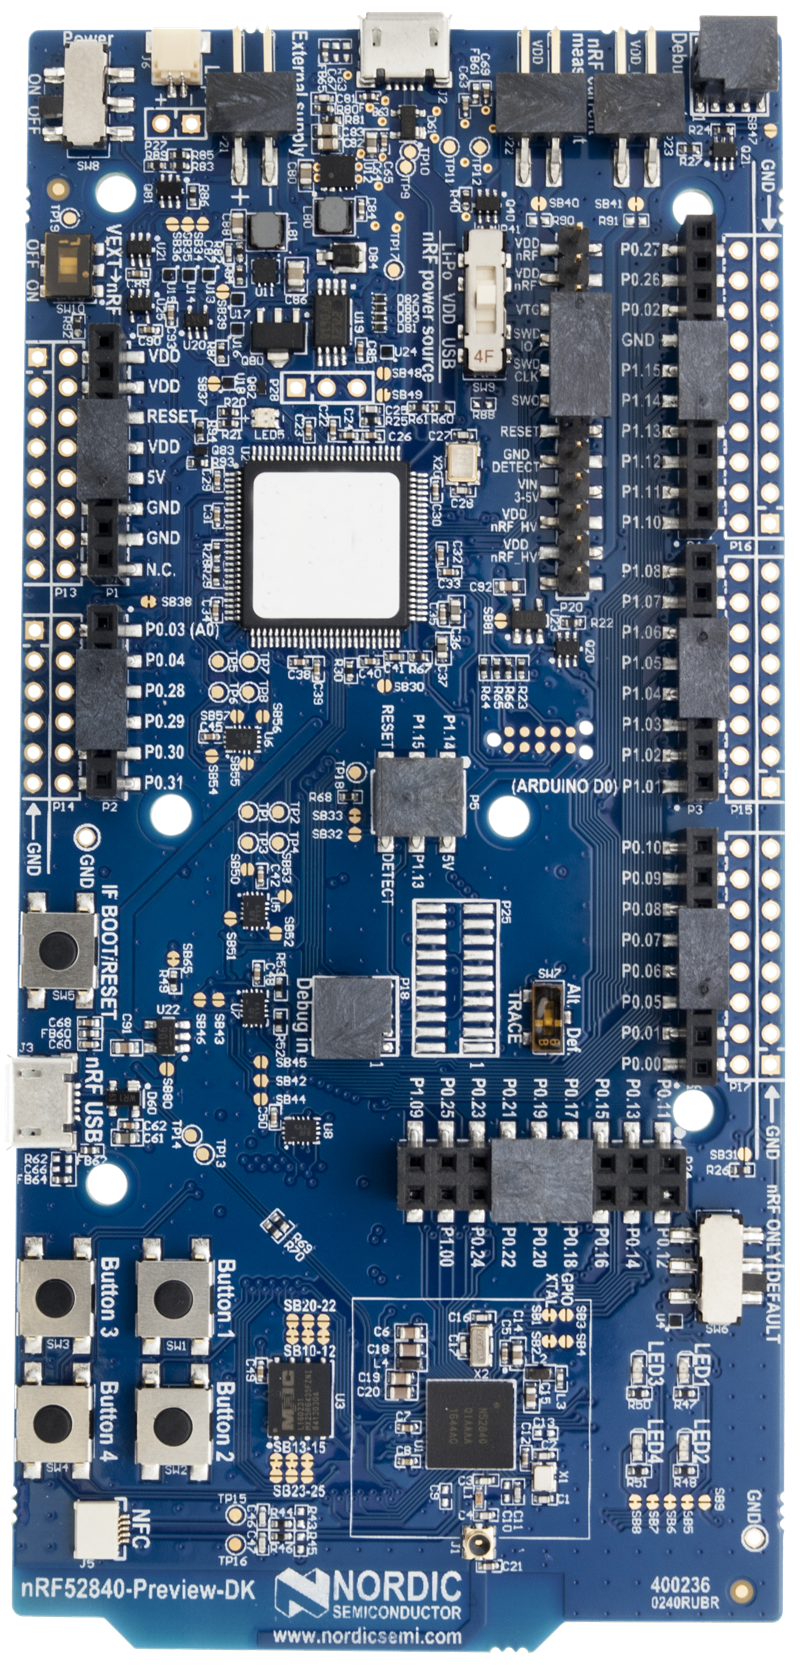
\includegraphics[scale=0.6]{figure/figure04_nRF52840.png}
    \caption{The nRF52840 DK.}
\end{figure}
\justify
The nRF52840 SoC is the most advanced member of the nRF52 series SoC family.
It has protocol support for Bluetooth 5, Bluetooth mesh, Thread, Zigbee, 
802.15.4, ANT and 2.4 GHz proprietary stacks. The nRF52840 is built around the 
32-bit Arm Cortex-M4 CPU with floating point unit running at 64 MHz. The flash and 
RAM size if 1 MB and 256 KB respectively, which is generous even for demanding 
applications. \cite{nrf19}
\justify
The Bluetooth protocol stack on the hardware is implemented as SoftDevice and 
distributed as a proprietary software. It is a Bluetooth Low Energy Central 
and Peripheral protocol stack solution which integrates a BLE Controller and 
Host and provides API for building BLE application. There also exists open-source BLE 
protocol stack implementation for the nRF52840, such as in the Zephyr project 
\cite{zep19}. However, for the ease of development, the SoftDevice is used along
with the provided nRF Software Development Kit (SDK).